\begin{frame}
	\frametitle{Não separação em arquivos}

	\begin{figure}[h]
		\centering
			
\includegraphics[height=0.6\paperheight]{figuras/hannah}
		\caption{Retirada do site \href{https://www.pensador.com/frase/MTE4NTA3Ng/}{Pensador}}\label{figure:hannah}
	\end{figure}

\end{frame}

\begin{frame}
	\frametitle{Problemas}

	\begin{itemize}
		\item Códigos "misturados"
	\end{itemize}

\end{frame}

\begin{frame}

	\Huge Exemplo

\end{frame}

\begin{frame}[fragile]

	\begin{listing}[H]
		\caption{Classe lidando com "escopos diferentes"}
		\begin{minted}[baselinestretch=1.2,fontsize=\scriptsize,linenos]{c++}
class ConexaoBancoDeDados{
	public:
		bool cadastrarProduto( Produto produto );
		bool cadastrarCliente( Cliente cliente );
		bool cadastrarUsuario( Usuario );

		Produto pegarInformacoesProduto( int idProduto );
		[...]
};
		\end{minted}
	\end{listing}

	\begin{listing}[H]
		\begin{minted}[baselinestretch=1.2,fontsize=\scriptsize,linenos]{c++}
conexaoBancoDeDados.cadastrarUsuario( usuario );
conexaoBancoDeDados.cadastrarCliente( cliente );
conexaoBancoDeDados.cadastrarProduto( produto );
		\end{minted}
	\end{listing}

\end{frame}

\begin{frame}[fragile]
	\frametitle{Solução}

	\begin{listing}[H]
		\begin{minted}[baselinestretch=1.0,fontsize=\scriptsize,linenos]{c++}
class ProdutoDAO : protected ConexaoBancoDeDados{
	public:
		bool cadastrar( Produto produto );
		Produto pegarInformacoes( id );
};

class ClienteDAO : protected ConexaoBancoDeDados{
	public:
		bool cadastrar( Cliente cliente );
		Cliente pegarInformacoes( int id );
};

class UsuarioDAO : protected ConexaoBancoDeDados{
	public:
		bool cadastrar( Usuario usuario );
		Usuario pegarInformacoes( int id );
};
		\end{minted}
	\end{listing}

	\begin{listing}[H]
		\begin{minted}[baselinestretch=1.2,fontsize=\scriptsize,linenos]{c++}
Produto produto = produtoDAO.pegarInformacoes( idProduto );
		\end{minted}
	\end{listing}

\end{frame}

\begin{frame}
	\frametitle{Exemplo de projeto em Java organizado de acordo com "proximidade"}

	\begin{figure}
		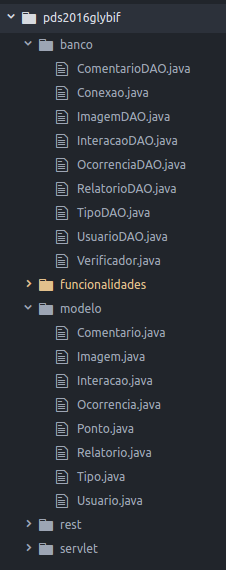
\includegraphics[width=0.22\textwidth]{figuras/organizacao}
		\label{figure:ProjetoOrganizado}
	\end{figure}

\end{frame}


\begin{frame}
	\frametitle{Solução}

	\begin{itemize}
		\item Agrupar as coisas (funções, classes, etc) de modo que as mesmas estejam juntas de acordo com sua proximidade
	\end{itemize}

\end{frame}
